%-----------------------------------------------------------------------------%
\section{Introduction}
An introduction in which the relevance of the project and its place in the context of geomatics is described, along with a clearly-defined problem statement.

"The Mystery of life is not a problem to solve, but a reality to experience"\cite{einstein}

    % \graphicspath{ {images/} }

\begin{figure}
    \centering
    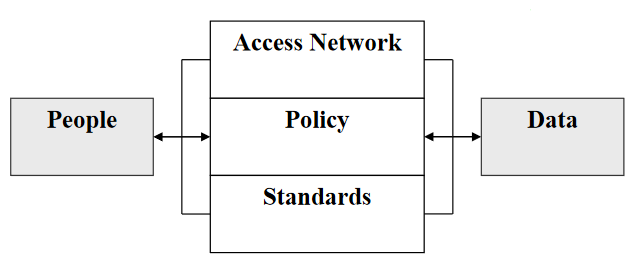
\includegraphics[width=12cm]{images/test.png}
    \caption{The main elements of an SDI}
    \label{thingie}
\end{figure}

as you can see at \reffig{thingie} 

%-----------------------------------------------------------------------------%

\section{Related work}
A related work section in which the relevant literature is presented and linked to the project.


%-----------------------------------------------------------------------------%
\section{Research questions}
The research questions are clearly defined, along with the scope (ie what you will not be doing).

To help you define a \"good\" research question, 
read \url{https://sites.duke.edu/urgws/files/2014/02/Research-Questions_WS-handout.pdf}.


%-----------------------------------------------------------------------------%
\section{Methodology}
Overview of the methodology to be used.

%-----------------------------------------------------------------------------%
\section{Time planning}
Having a Gantt chart is probably a better idea then just a list.

%-----------------------------------------------------------------------------%
\section{Tools and datasets used}
Since specific data and tools have to be used, it’s good to present these concretely, 
so that the mentors know that you have a grasp of all aspects of the project.
